%\documentclass{standalone}
%\usepackage{tikz}
%\begin{document}
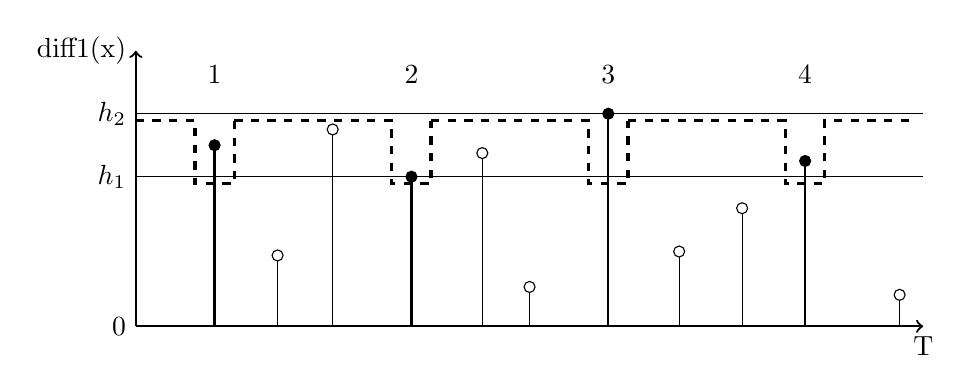
\begin{tikzpicture}[scale = 1.0]
\def\h{1.3}
\def\m{2.5}
% DELTA ADN SHIFT
\def\d{0.25}
\def\s{0.09}
\draw[->, thick] (0,0) -- (10, 0);
\draw[->, thick] (0,0) -- (0, 3.5);
\node [below, minimum size = 0.25cm] at (10,0) {T};
\node [left, minimum size = 0.25cm] at (0,3.5) {diff1(x)};
\node [left] at (0, 0) {0};
% TPs
\draw[thick] (1, 0)          -- (1         , 2.3);
\draw[thick] (1 + \m, 0)     -- (1 + \m    , 1.9);
\draw[thick] (1 + 2 * \m, 0) -- (1 + 2 * \m, 2.7);
\draw[thick] (1 + 3 * \m, 0) -- (1 + 3 * \m, 2.1);
% TP circles
\draw[fill=black] (1, 2.3) circle (0.07);
\draw[fill=black] (1+\m, 1.9) circle (0.07);
\draw[fill=black] (1+2*\m, 2.7) circle (0.07);
\draw[fill=black] (1+3*\m, 2.1) circle (0.07);
% TPS text
\node at (1       , 3.2) {1};
\node at (1 + \m  , 3.2) {2};
\node at (1 + 2*\m, 3.2) {3};
\node at (1 + 3*\m, 3.2) {4};
% RANGE / BAND
\draw (0, 1.9) -- (10.0, 1.9);
\draw (0, 2.7) -- (10.0, 2.7);
\node [left] at (0, 1.9) {$h_1$};
\node [left] at (0, 2.7) {$h_2$};
%FAs
\draw (1.8, 0) -- (1.8, 0.9);
\draw (2.5, 0) -- (2.5, 2.5);
\draw (1 + \m + 0.9, 0) -- (1 + \m + 0.9, 2.2);
\draw (1 + \m + 1.5, 0) -- (1 + \m + 1.5, 0.5);
\draw (1 + 2 * \m + 0.9, 0) -- (1 + 2 * \m + 0.9, 0.95);
\draw (1 + 2 * \m + 1.7, 0) -- (1 + 2 * \m + 1.7, 1.5);
\draw (1 + 3 * \m + 1.2, 0) -- (1 + 3 * \m + 1.2, 0.4);
% FAs circles
\draw[fill=white] (1.8, 0.9) circle (0.07);
\draw[fill=white] (2.5, 2.5) circle (0.07);
\draw[fill=white] (1+\m + 0.9, 2.2) circle (0.07);
\draw[fill=white] (1+\m + 1.5, 0.5) circle (0.07);
\draw[fill=white] (1+2*\m + 0.9, 0.95) circle (0.07);
\draw[fill=white] (1+2*\m + 1.7, 1.5) circle (0.07);
\draw[fill=white] (1+3*\m + 1.2, 0.4) circle (0.07);
% OPTIMAL DYNAMIC H
\draw[dashed, line width=1.2pt] (0, 2.7 - \s) -- (1 - \d, 2.7- \s) -- (1 - \d, 1.9 - \s) -- (1 + \d, 1.9 - \s) -- (1 + \d, 2.7 - \s);
\draw[dashed, line width=1.2pt] (1 + \d, 2.7 - \s) -- (1 + \m - \d, 2.7 - \s) -- (1 + \m - \d, 1.9 - \s) -- (1 + \m + \d, 1.9 - \s) -- (1 + \m + \d, 2.7 - \s);
\draw[dashed, line width=1.2pt] (1 + \m + \d, 2.7 - \s) -- (1+2*\m-\d, 2.7-\s) -- (1+2*\m-\d, 1.9-\s) -- (1+2*\m+\d, 1.9-\s) -- (1+2*\m+\d, 2.7-\s);
\draw[dashed, line width=1.2pt] (1+2*\m+\d, 2.7-\s) -- (1+3*\m - \d, 2.7-\s) -- (1+3*\m - \d, 1.9-\s) -- (1+3*\m + \d, 1.9-\s) -- (1+3*\m + \d, 2.7-\s) -- (1 + 3*\m + 1.4, 2.7 - \s);
\end{tikzpicture}
%\end{document}
